\PassOptionsToPackage{dvipsnames}{xcolor}
\PassOptionsToPackage{unicode}{hyperref}
\PassOptionsToPackage{naturalnames}{hyperref}
\documentclass[aspectratio=169,10pt]{beamer}

% language and encoding
\usepackage[french]{babel}
\usepackage[T1]{fontenc}
\usepackage{csquotes}

% biblatex for references on slides
% TODO: short format in footnotes (cf. https://tex.stackexchange.com/a/215608)
\usepackage[backend=biber,bibencoding=utf8,style=verbose-inote,citestyle=authortitle]{biblatex}
\addbibresource{defense.bib}
% \usepackage{xpatch}
% \xapptobibmacro{cite}{\setunit{\nametitledelim}\printfield{title}}{}{}
% another way? https://tex.stackexchange.com/a/653833

% beamer theme
\usetheme{moloch}
\usepackage{appendixnumberbeamer}
\usepackage{fontspec}
\setsansfont[
  ItalicFont={Fira Sans Light Italic},
  BoldFont={Fira Sans},
  BoldItalicFont={Fira Sans Italic}
]{Fira Sans Light}
\setmonofont[BoldFont={Fira Mono Medium}]{Fira Mono}
\AtBeginEnvironment{tabular}{%
  \addfontfeature{Numbers={Monospaced}}
}
% https://steeven9.github.io/USI-LaTeX/html/packages_hyperref_babel_xcolor3.html
% Section 3.2 of:
% https://mirror.ibcp.fr/pub/CTAN/macros/latex/contrib/beamer-contrib/themes/moloch/moloch.pdf
\setbeamercolor{progress bar}{fg=BrickRed}
\setbeamercolor{title separator}{fg=BrickRed}
% footnote font size
\setbeamerfont{footnote}{size=\tiny}
% solid background for blocks
\molochset{block=fill}
% remove section frames
% \molochset{sectionpage=none}
% smaller first-level bullet points
\setbeamertemplate{itemize item}{\textbullet}

% figures uncover animation (cf. https://tex.stackexchange.com/a/354033/95423)
\setbeamercovered{transparent}
\newcommand<>{\uncovergraphics}[2][{}]{
    \begin{tikzpicture}
    \node[anchor=south west,inner sep=0] (B) at (4,0)
        {\includegraphics[#1]{#2}};
    \alt#3{}{%
        \fill [draw=none, fill=background, fill opacity=0.9] (B.north west) -- (B.north east) -- (B.south east) -- (B.south west) -- (B.north west) -- cycle;
    }
    \end{tikzpicture}
}

% fonts and symbols
\usepackage{pifont}
\newcommand{\cmark}{\color{YellowGreen}\ding{51}}
\newcommand{\xmark}{\color{BrickRed}\ding{55}}
\usepackage{textcomp}
\usepackage{emoji}
% math
\usepackage{amsmath,amssymb,amsfonts}
% links
\usepackage{hyperref}
% tables
\usepackage{tabularx}
\usepackage{booktabs}
% various tabular columns with text wrapping
\newcolumntype{L}{>{\arraybackslash}m{\linewidth}}
\newcolumntype{M}{>{\centering\arraybackslash}m{0.33\linewidth}}
\newcolumntype{Y}{>{\centering\arraybackslash}m{0.15\linewidth}}
\newcolumntype{y}{>{\arraybackslash}m{0.15\linewidth}}
% generic horizontally centered column with line breaks
\newcolumntype{Z}{>{\centering\arraybackslash}X}
% vertical centering of text in all tabularx columns
\renewcommand\tabularxcolumn[1]{m{#1}}

% redefine title page
% https://tex.stackexchange.com/a/396409
% Section 6.2.3 of:
% https://ctan.math.illinois.edu/macros/latex/contrib/beamer-contrib/themes/moloch/moloch.pdf
\makeatletter
\setbeamertemplate{title page}{
  \begin{minipage}[b][\paperheight]{\textwidth}
    % \vfill%
    \ifx\inserttitle\@empty\else\usebeamertemplate*{title}\fi
    \ifx\insertsubtitle\@empty\else\usebeamertemplate*{subtitle}\fi
    \vspace{.2cm}
    \ifx\insertdate\@empty\else\usebeamertemplate*{date}\fi
    \usebeamertemplate*{title separator}
    \vspace{-.2cm}
    \begin{columns}[]
        \column{0.4\linewidth}
        \ifx\beamer@shortauthor\@empty\else\usebeamertemplate*{author}\fi
        \column{0.4\linewidth}
        % \begin{table}[]
        %     \begin{flushleft}
        %         \small
        %         \begin{tabular}{ll}
        %             Rapporteur & Blabla \\
        %             Rapporteur & Blabla
        %         \end{tabular}
        %     \end{flushleft}
        % \end{table}
    \end{columns}
    \begin{columns}[b]
        \column{0.4\linewidth}
        \ifx\insertinstitute\@empty\else\usebeamertemplate*{institute}\fi
        \column{0.5\linewidth}
        \ifx\inserttitlegraphic\@empty\else\inserttitlegraphic\fi
    \end{columns}
    \vspace*{.2cm}
  \end{minipage}
}
\makeatother

\title{Allocation et placement dynamiques sur ressources hétérogènes pour le cloud serverless}
% \subtitle{}
\date{\today}
\titlegraphic{\flushright\includegraphics[height=1cm]{img/logos.png}\vspace{.5cm}}

\author{
    \texorpdfstring{
        \begin{table}[]
            \begin{flushleft}
                \begin{tabular}{ll}
                    Thèse soutenue par   & \textbf{Vincent Lannurien}~\inst{1, 2} \\
                                         & \\
                    Sous la direction de & Jalil Boukhobza~\inst{1, 2} \\
                    Co-dirigée par       & Laurent D'Orazio~\inst{1, 3} \\
                                         & Olivier Barais~\inst{1, 3} \\
                    Encadrée par         & Stéphane Paquelet~\inst{1}
                \end{tabular}
            \end{flushleft}
        \end{table}
    }
    {
        Vincent Lannurien \and
        Jalil Boukhobza \and
        Laurent D'Orazio \and
        Olivier Barais \and
        Stéphane Paquelet
    }
}

\institute{
    \texorpdfstring{
        \begin{table}[]
            \centering
            \begin{flushleft}
                \begin{tabular}{L}
                    \inst{1} b{\textless\textgreater}com Institute of Research and Technology \\
                    \inst{2} ENSTA Bretagne, Lab-STICC, CNRS, UMR 6285 \\
                    \inst{3} Univ. Rennes, Inria, CNRS, IRISA
                \end{tabular}
            \end{flushleft}
        \end{table}
    }
    {
        b{\textless\textgreater}com Institute of Research and Technology \and
        ENSTA Bretagne, Lab-STICC, CNRS, UMR 6285 \and
        Univ. Rennes, Inria, CNRS, IRISA
    }
}

\begin{document}

\maketitle

\begin{frame}{Introduction}
    \begin{center}
        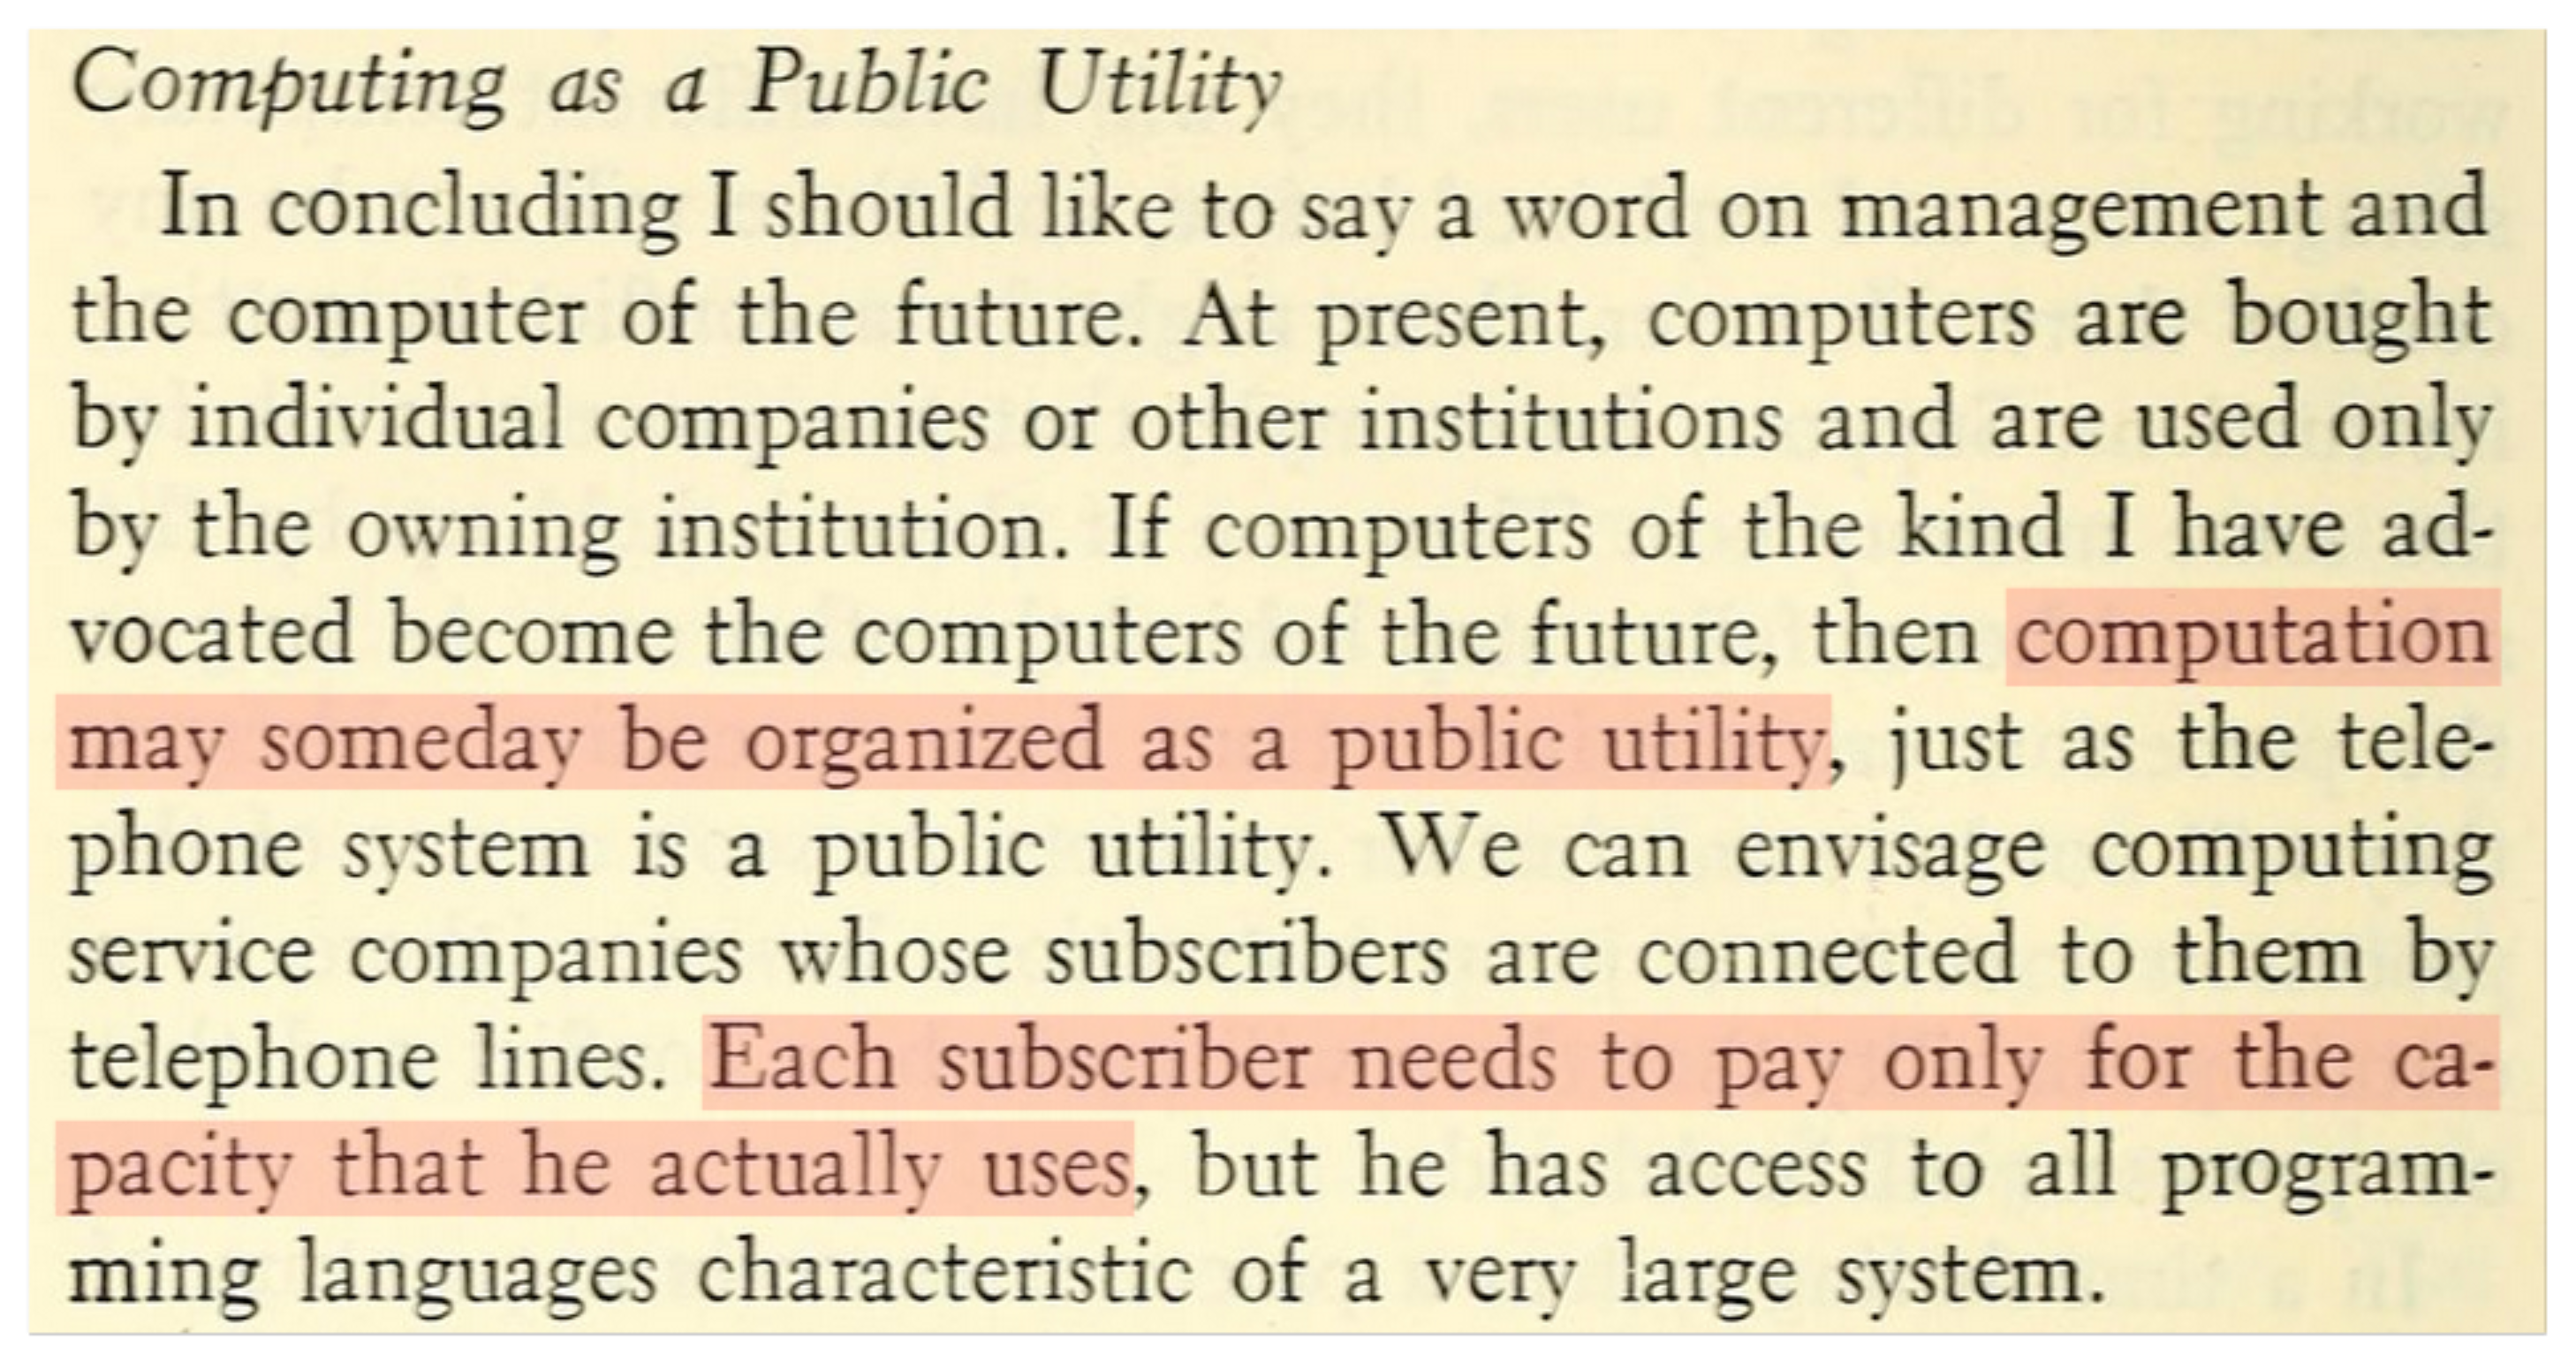
\includegraphics[width=0.8\textwidth]{img/mccarthy.png}
    \end{center}

    \addtocounter{footnote}{1}
    \footnotetext{\fullcite{greenberger1962management}}
\end{frame}

\begin{frame}{Plan de la présentation}
    \begin{columns}[c,onlytextwidth]
        \column{0.45\textwidth}
        \setbeamertemplate{section in toc}[sections numbered]
        \tableofcontents[hideallsubsections]

        \column{0.45\textwidth}
        \begin{center}
            \includegraphics[width=\columnwidth]{img/toc.png}
        \end{center}
    \end{columns}
\end{frame}

\section{Contexte et état de l'art}

\begin{frame}{\textit{Cloud computing}}
    \begin{columns}
        \column{0.45\textwidth}
        \begin{itemize}
            \item Définition donnée par le NIST~\footnotemark{} :
            \begin{itemize}
                \item Service \textbf{à la demande} ;
                \item \textbf{Accessible} par le réseau ;
                \item Ressources \textbf{partagées} ;
                \item \textbf{Élasticité} rapide ;
                \item Service \textbf{mesuré}.
            \end{itemize}
        \end{itemize}

        \begin{center}
            \includegraphics[width=0.8\columnwidth]{img/cloud-scaling.png}
        \end{center}

        \column{0.45\textwidth}
        \begin{center}
            \includegraphics[width=\columnwidth]{img/cloud.png}
        \end{center}
    \end{columns}

    \footnotetext{\fullcite{mellNISTDefinitionCloud}}
    \addtocounter{footnote}{1}
    \footnotetext{\fullcite{wilder2012cloud}}
\end{frame}

\begin{frame}{Problématique : dimensionnement}
    \begin{columns}
        \column{0.5\textwidth}
        \begin{itemize}
            \item Dimensionnement aux pics
            \begin{itemize}
                \item \textit{Over provisioning}
            \end{itemize}
            \item Exigences de QoS
            \begin{itemize}
                \item \textit{Over committing}
            \end{itemize}
            \item Ressources dormantes
            \begin{itemize}
                \item \textit{Under utilization}
            \end{itemize}
        \end{itemize}

        \begin{center}
            \includegraphics[width=\columnwidth]{img/dimensionnement-1.png}
        \end{center}

        \column{0.5\textwidth}
        \begin{center}
            \includegraphics[width=\columnwidth]{img/dimensionnement-2.png}
        \end{center}
    \end{columns}

    \addtocounter{footnote}{1}
    \footnotetext{\fullcite{armbrustViewCloudComputing2010}}
    \addtocounter{footnote}{1}
    \footnotetext{\fullcite{bitingoff_ghosh_2012}}
\end{frame}

\begin{frame}{Problématique : consommation d'énergie}
    \begin{columns}
        \column{0.5\textwidth}
        \begin{itemize}
            \item Énergie dans le cloud :
            \begin{itemize}
                \item $\sim$ 1,5\% de la consommation mondiale ;
                \item $\sim$ 2,7\% de la consommation en Europe ;
                \item ...
            \end{itemize}
            \item Bilan carbone du numérique :
            \begin{itemize}
                \item Leviers : fabrication, utilisation~\footnotemark{}
            \end{itemize}
        \end{itemize}

        \column{0.5\textwidth}
    \end{columns}

    \footnotetext{\fullcite{Numerique40Budget2021}}
\end{frame}

\begin{frame}{Problématique : hétérogénéité matérielle}
    ... (diagramme de Venn)
\end{frame}

\begin{frame}{\textit{Serverless computing} : une définition}
    \begin{columns}
        \column{0.5\textwidth}
        \begin{itemize}
            \item Une nouvelle abstraction pour le cloud :
            \begin{itemize}
                \item Unité d'allocation : \textbf{temps} plutôt que \textbf{ressource} ;
                \item Granularité fine : déploiement de \textbf{fonctions} ;
                \item Déplacement de la responsabilité : de l'utilisateur vers le fournisseur de services.
            \end{itemize}
        \end{itemize}

        \column{0.5\textwidth}
        \begin{center}
            \includegraphics[width=\columnwidth]{img/serverless.png}
        \end{center}
    \end{columns}

    \footnotetext{\fullcite{SchleierSmith2021WhatSC}}
\end{frame}

\begin{frame}{\textit{Serverless computing} : défis}
    \begin{itemize}[<+- | alert@+>]
        \item Les ressources matérielles ne sont \textit{pas réservées}~\footfullcite{SchleierSmith2021WhatSC}
        \begin{itemize}
            \item Responsabilité accrue pour le fournisseur de services
            \begin{itemize}
                \item \textbf{Allocation} dynamique (en fonction des variations de charge)
                \item \textbf{Placement} dynamique (des requêtes sur les ressources)
            \end{itemize}
        \end{itemize}

        \item Cloud resources are \textit{heterogeneous}~\footfullcite{hortaXartrekRuntimeExecution2021}
        \begin{itemize}
            \item Différents niveaux de \textbf{performance}
            \item Différents profils de \textbf{coût}
        \end{itemize}

        \item La charge est \textit{difficilement prévisible}~\footfullcite{shahradServerlessWildCharacterizing}
        \begin{itemize}
            \item Barrière stochastique
            \item L'orchestration est un processus en ligne
        \end{itemize}

        \item Les utilisateurs ont des besoins en \textit{QoS variés}~\footfullcite{buyyaSLAorientedResourceProvisioning2011}
        \begin{itemize}
            \item Certains cas d'usage requièrent un haut débit (tâches en lots)
            \item D'autres sont sensibles à la latence (applications interactives)
        \end{itemize}
    \end{itemize}
\end{frame}

\begin{frame}{\textit{Serverless computing} : opportunités et menaces}
    \begin{center}
        \textbf{Garantir la Qualité de Service pour des ressources hétérogènes non réservées}

        \begin{table}[]
            \centering
            \begin{tabularx}{\textwidth}{ZZ}
                \toprule
                \addlinespace[0.5em]
                \textbf{Opportunité} & \textbf{Menace} \\
                \addlinespace[0.5em]
                \midrule
                \addlinespace[0.5em]
                \textbf{Dimensionnement dynamique} pour aligner l'usage des ressources sur le besoin réel & \textbf{Pics de latence} liés au démarrage à froid des fonctions \\
                \addlinespace[0.5em]
                \midrule
                \addlinespace[0.5em]
                \textbf{Placement optimal} des requêtes utilisateur sur les instances de fonctions & \textbf{Baisses de débit} liées aux communications sur stockage lent pour la composition de fonctions \\
                \addlinespace[0.5em]
                \bottomrule
            \end{tabularx}
        \end{table}
    \end{center}
\end{frame}

\section{HeROfake : Orchestration serverless sur ressources hétérogènes pour le cloud privé}

\begin{frame}{}
    \begin{exampleblock}{Question de recherche 1 (\textbf{QR1})}
        Comment dimensionner les allocations dynamiques de ressources hétérogènes pour une application simple, constituée de fonctions de courte durée, et comment ordonnancer efficacement les requêtes des utilisateurs, lorsque ces derniers ont des besoins variés en matière de qualité de service ?
    \end{exampleblock}
\end{frame}

\section{HeROcache : Applications serverless et coûts associés aux systèmes de stockage}

\begin{frame}{}
    \begin{exampleblock}{Question de recherche 2 (\textbf{QR2})}
        Comment déployer des applications complexes, composées de chaînes de fonctions de courte durée, et comment tirer parti de l'hétérogénéité des nœuds disponibles à l'edge, pour respecter la qualité de service requise par les utilisateurs tout en contenant la consommation d'énergie de l'infrastructure ?
    \end{exampleblock}
\end{frame}

\section{HeROsim : Élaborer et évaluer des politiques d'orchestration serverless}

\begin{frame}{}
    \begin{exampleblock}{Question de recherche 3 (\textbf{QR3})}
        Du point de vue d'un fournisseur de services pour le cloud, comment évaluer et comparer l'impact sur la qualité de service de différentes politiques d'allocation de ressources et d'ordonnancement de tâches dans le modèle serverless ?
    \end{exampleblock}
\end{frame}

\section{Conclusion}

\subsection{Résumé}

\begin{frame}{}
    ...
\end{frame}

\subsection{Perspectives}

\begin{frame}{}
    ...
\end{frame}

\begin{frame}[standout]
    Merci de votre attention.
\end{frame}

\appendix

\begin{frame}[allowframebreaks]{References}
    \printbibliography[heading=none]
\end{frame}

\end{document}
